% mnras_template.tex 
%
% LaTeX template for creating an MNRAS paper
%
% v3.3 released April 2024
% (version numbers match those of mnras.cls)
%
% Copyright (C) Royal Astronomical Society 2015
% Authors:
% Keith T. Smith (Royal Astronomical Society)

% Change log
%
% v3.3 April 2024
%   Updated \pubyear to print the current year automatically
% v3.2 July 2023
%	Updated guidance on use of amssymb package
% v3.0 May 2015
%    Renamed to match the new package name
%    Version number matches mnras.cls
%    A few minor tweaks to wording
% v1.0 September 2013
%    Beta testing only - never publicly released
%    First version: a simple (ish) template for creating an MNRAS paper

%%%%%%%%%%%%%%%%%%%%%%%%%%%%%%%%%%%%%%%%%%%%%%%%%%
% Basic setup. Most papers should leave these options alone.
\documentclass[fleqn,usenatbib]{mnras}

% MNRAS is set in Times font. If you don't have this installed (most LaTeX
% installations will be fine) or prefer the old Computer Modern fonts, comment
% out the following line
\usepackage{newtxtext,newtxmath}
% Depending on your LaTeX fonts installation, you might get better results with one of these:
%\usepackage{mathptmx}
%\usepackage{txfonts}

% Use vector fonts, so it zooms properly in on-screen viewing software
% Don't change these lines unless you know what you are doing
\usepackage[T1]{fontenc}

% Allow "Thomas van Noord" and "Simon de Laguarde" and alike to be sorted by "N" and "L" etc. in the bibliography.
% Write the name in the bibliography as "\VAN{Noord}{Van}{van} Noord, Thomas"
\DeclareRobustCommand{\VAN}[3]{#2}
\let\VANthebibliography\thebibliography
\def\thebibliography{\DeclareRobustCommand{\VAN}[3]{##3}\VANthebibliography}


%%%%% AUTHORS - PLACE YOUR OWN PACKAGES HERE %%%%%

% Only include extra packages if you really need them. Avoid using amssymb if newtxmath is enabled, as these packages can cause conflicts. newtxmatch covers the same math symbols while producing a consistent Times New Roman font. Common packages are:
\usepackage{graphicx}	% Including figure files
\usepackage{amsmath}	% Advanced maths commands

%%%%%%%%%%%%%%%%%%%%%%%%%%%%%%%%%%%%%%%%%%%%%%%%%%

%%%%% AUTHORS - PLACE YOUR OWN COMMANDS HERE %%%%%

% Please keep new commands to a minimum, and use \newcommand not \def to avoid
% overwriting existing commands. Example:
%\newcommand{\pcm}{\,cm$^{-2}$}	% per cm-squared

%%%%%%%%%%%%%%%%%%%%%%%%%%%%%%%%%%%%%%%%%%%%%%%%%%

%%%%%%%%%%%%%%%%%%% TITLE PAGE %%%%%%%%%%%%%%%%%%%

% Title of the paper, and the short title which is used in the headers.
% Keep the title short and informative.
\title{Detecting the self-lensing black hole population}

% The list of authors, and the short list which is used in the headers.
% If you need two or more lines of authors, add an extra line using \newauthor
\author[Adam McMaster et al.]{
Adam McMaster,$^{1}$\thanks{E-mail: a.mcmaster@soton.ac.uk}
A. N. Other,$^{2}$
Third Author$^{2,3}$
and Fourth Author$^{3}$
\\
% List of institutions
$^{1}$University of Southampton...\\
$^{2}$Department, Institution, Street Address, City Postal Code, Country\\
$^{3}$Another Department, Different Institution, Street Address, City Postal Code, Country
}

% These dates will be filled out by the publisher
\date{Accepted XXX. Received YYY; in original form ZZZ}

% Prints the current year, for the copyright statements etc. To achieve a fixed year, replace the expression with a number. 
\pubyear{\the\year{}}

% Don't change these lines
\begin{document}
\label{firstpage}
\pagerange{\pageref{firstpage}--\pageref{lastpage}}
\maketitle

% Abstract of the paper
\begin{abstract}
This is a simple template for authors to write new MNRAS papers.
The abstract should briefly describe the aims, methods, and main results of the paper.
It should be a single paragraph not more than 250 words (200 words for Letters).
No references should appear in the abstract.
\end{abstract}

% Select between one and six entries from the list of approved keywords.
% Don't make up new ones.
\begin{keywords}
keyword1 -- keyword2 -- keyword3
\end{keywords}

%%%%%%%%%%%%%%%%%%%%%%%%%%%%%%%%%%%%%%%%%%%%%%%%%%

%%%%%%%%%%%%%%%%% BODY OF PAPER %%%%%%%%%%%%%%%%%%

\section{Introduction}

Paper aims:
\begin{enumerate}
    \item Produce a library of ``pristine'' simulated self-lensing light curves and RV curves, covering all plausible physical parameter space.
    \item Simulate observing those systems under a range of observing schedules (a small number of representative schedules, not fully comprehensive as it'll be too much) and with a variety of instrument accuracies.
    \item Fit simulated observations and determine which parameters can and can not be recovered as a function of instrument accuracies, for each observing schedule.
    \item Combine these results with previous population synthesis results to determine how many such systems could be discovered by each instrument/strategy.
\end{enumerate}

The main distinguishing feature of self-lensing vs microlensing is the periodicity of the lensing flares. To claim photometric discovery of a self-lensing system, ideally we would aim to detect this periodicity. 

\section{Methods}

\subsection{``Pristine'' simulations}

Describe py-self-lensing code and maths behind LC and RV

We compute photometric light curves and RV curves with no noise for a grid of parameter values.  We assume the stellar companion is Sun-like (1 M$_\odot$, 1 R$_\odot$, 5500 K). Other params are sampled linearly spaced as follows:

\begin{itemize}
    \item $a$ (semi-major axis): 10 samples between 0.1 and 5 AU, 10 samples between 5 and 50 AU, 10 samples between 50 and 200 AU.
    \item $M_\text{BH}$: 10 samples between 5 and 50 M$_\odot$.
    \item $e$ (eccentricity): 10 samples between 0 and 0.9.
    \item $\omega$ (periapsis phase angle; 0 meaning closest approach at peak of lensing): 10 samples between 0 and $2\pi$.
\end{itemize}

We exclude from above any combination of $a$ and $M_\text{BH}$ where the Roche lobe radius at periapsis would be smaller than or equal to 1~R$_\odot$, as such systems would be guaranteed to be X-ray binaries.

Three photometric effects are included when generating the light curves: self-lensing, ellipsoidal variations, and Doppler boosting. At small values of $a$ the light curve is dominated by ellipsoidal variations and Doppler boosting (though lensing is often visible too); at large $a$ lensing is dominant, with ellipsoidal variation and Doppler boosting tending to zero as $a$ increases.

Calculation of self-lensing magnifications is performed according to the lensing formulae given by \cite{witt_can_1994}, with source-lens distance calculated assuming a Keplerian orbit with the given semi-major axis, BH mass, eccentricity, and periapsis phase angle. Calculation of ellipsoidal variations and Doppler boosting, and the combination of these effects with self-lensing, follow \cite{sorabella_modeling_2022}, with the addiition of a variable orbital separation to account for eccentricity in the ellipsoidal variation calculation. These effects all depend on the orbital phase at a given time during the simulation. The zero point for this is defined as the moment of maximum lensing magnification (i.e. the time of minimum separation between source and lens, $t_0$). The periapsis phase angle is defined in terms of this zero point; i.e. the phase angle at which periastron passage occurs, relative to the position at $t_0$. The source-lens distance is calculated for each time according to the phase angle at that time, meaning the source-lens distance changes during the microlensing event according to the eccentricity. Strictly speaking, the Einstein ring radius should also change as a function of orbital phase, but this is not accounted for in the present work. Instead, the radius at $t_0$ is used for all calculations.

\subsection{Simulated realistic observations}

Observing strategy. Instrument accuracies.

Assumptions: We first identify lensing candidates in photometry some time after the event, and then obtain RV after that. For simplicity we assume that there is a gap of one year between first photometric lensing event and the RV being obtained.

We simulate varying lengths of photometric light curve, varying lengths of RV curves, varying observing cadences for both LC and RV. Done by sampling the pristine simulations at different frequencies.

For a sufficiently close binary, a self-lensing system would be indistinguishable from a binary undergoing ellipsoidal variations with no self-lensing effect, since the lensing magnification would so small as to be undetectable. Indeed the only physical difference is the angle of inclination; there is no inherent difference between the two classes of system. In this work we assume all systems are edge-on.

\subsection{Fitting of simulated observations}

We detect potential periodicity with Lomb-Scargle. All periods up to 90\% of observing baseline with powers above 99\% FAL are considered and used to apply a Gaussian prior in MCMC. Fitted periods longer than 90\% of observing baseline are allowed with no Gaussian prior, with a maximum of double the observing baseline. 

In other words, if fitting a period shorter than 90\% of baseline we're strict about it fitting close to one of the Lomb-Scargle periods; if it's that short we enforce that we should see one or more full orbits in the photometry. We then enforce an overall limit on orbital period of twice the baseline. These measures are both designed to force the fitted parameters into a range where we can be confident in them based on the length of the photometic basline. E.g. if we only have a year of photometry, we shouldn't claim to be able to see a SL system with a 5 year orbit. For reliability we should get more photometry to make that claim. And conversely if we have a year of photometry and the orbital period is a month, it should show up in the Lomb-Scargle results.

\subsection{Combining with pop synthesis}

\section{Results}

\subsection{Pristine RV curves}

Generated RV curves with no added noise and assuming one measurement per day.

% \begin{figure}
%     \centering
%     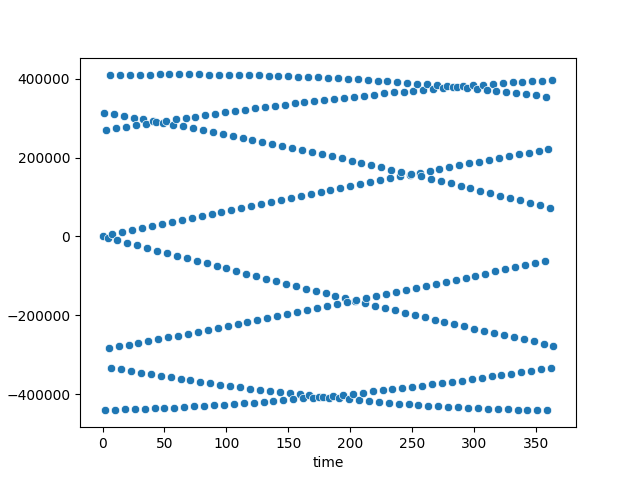
\includegraphics[width=\linewidth]{plots/pristine/0.1/0.1111111111111111/3.490658503988659/18.788888888888888/unfolded.png}
%     \caption{A simulated RV curve for a self-lensing system with $a = 0.1$ AU, $e = 0.1$, and $M_\text{tot} = 18.7 \text{M}_\odot$, shows a year's worth of daily RV measurements.}
%     \label{fig:pristine-rv-unfolded}
% \end{figure}

% \begin{figure}
%     \centering
%     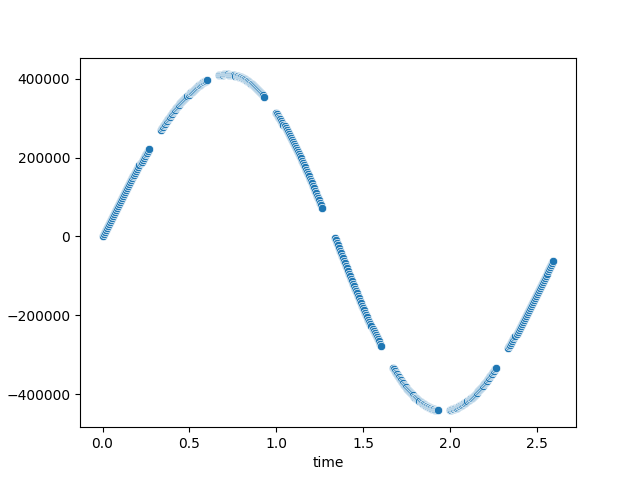
\includegraphics[width=\linewidth]{plots/pristine/0.1/0.1111111111111111/3.490658503988659/18.788888888888888/folded.png}
%     \caption{The RV curve from Figure~\ref{fig:pristine-rv-unfolded} folded at its orbital period.}
%     \label{fig:pristine-rv-folded}
% \end{figure}


% \begin{figure}
%     \centering
%     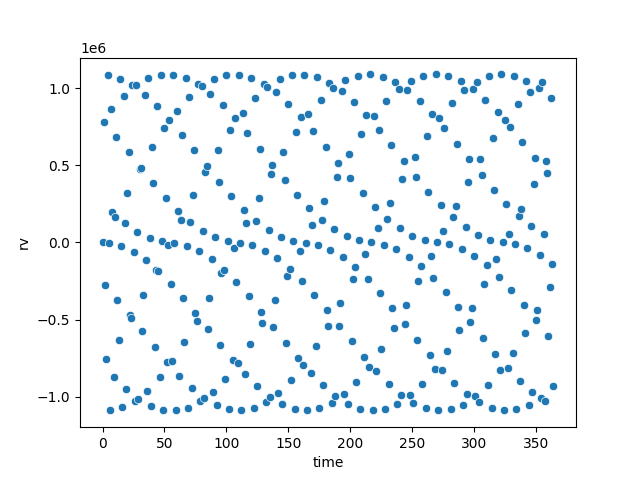
\includegraphics[width=\linewidth]{plots/pristine/0.1/0.8888888888888888/0.0/12.155555555555553/unfolded.png}
%     \caption{A simulated RV curve for a self-lensing system with $a = 0.1$ AU, $e = 0.89$, and $M_\text{tot} = 12.16 \text{M}_\odot$, shows a year's worth of daily RV measurements.}
%     \label{fig:pristine-rv-eccentric-unfolded}
% \end{figure}

% \begin{figure}
%     \centering
%     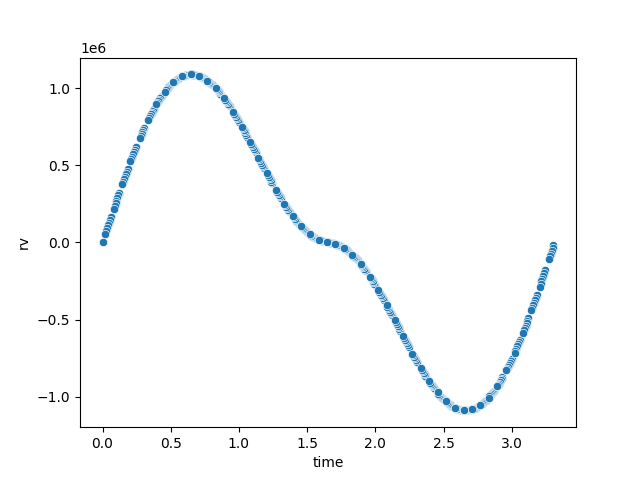
\includegraphics[width=\linewidth]{plots/pristine/0.1/0.8888888888888888/0.0/12.155555555555553/folded.png}
%     \caption{The RV curve from Figure~\ref{fig:pristine-rv-eccentric-unfolded} folded at its orbital period.}
%     \label{fig:pristine-rv-eccentric-folded}
% \end{figure}


\section{Discussion}



\section{Conclusions}

The last numbered section should briefly summarise what has been done, and describe
the final conclusions which the authors draw from their work.

\section*{Acknowledgements}

The Acknowledgements section is not numbered. Here you can thank helpful
colleagues, acknowledge funding agencies, telescopes and facilities used etc.
Try to keep it short.

%%%%%%%%%%%%%%%%%%%%%%%%%%%%%%%%%%%%%%%%%%%%%%%%%%
\section*{Data Availability}

 
The inclusion of a Data Availability Statement is a requirement for articles published in MNRAS. Data Availability Statements provide a standardised format for readers to understand the availability of data underlying the research results described in the article. The statement may refer to original data generated in the course of the study or to third-party data analysed in the article. The statement should describe and provide means of access, where possible, by linking to the data or providing the required accession numbers for the relevant databases or DOIs.




%%%%%%%%%%%%%%%%%%%% REFERENCES %%%%%%%%%%%%%%%%%%

% The best way to enter references is to use BibTeX:

\bibliographystyle{mnras}
\bibliography{example} % if your bibtex file is called example.bib


% Alternatively you could enter them by hand, like this:
% This method is tedious and prone to error if you have lots of references
%\begin{thebibliography}{99}
%\bibitem[\protect\citeauthoryear{Author}{2012}]{Author2012}
%Author A.~N., 2013, Journal of Improbable Astronomy, 1, 1
%\bibitem[\protect\citeauthoryear{Others}{2013}]{Others2013}
%Others S., 2012, Journal of Interesting Stuff, 17, 198
%\end{thebibliography}

%%%%%%%%%%%%%%%%%%%%%%%%%%%%%%%%%%%%%%%%%%%%%%%%%%

%%%%%%%%%%%%%%%%% APPENDICES %%%%%%%%%%%%%%%%%%%%%

\appendix

\section{Some extra material}

If you want to present additional material which would interrupt the flow of the main paper,
it can be placed in an Appendix which appears after the list of references.

%%%%%%%%%%%%%%%%%%%%%%%%%%%%%%%%%%%%%%%%%%%%%%%%%%


% Don't change these lines
\bsp	% typesetting comment
\label{lastpage}
\end{document}

% End of mnras_template.tex
